\section{Химические источники тока, их классификация. Электролиз растворов и расплавов.}
	Почти все это и не только можно найти в Еремине стр 104.
	Если в окислительно восстановительной реакции пространственно разделить процесс восстановления окислители и окисления восстановителя, то мы получим электрический ток по тому каналу, где пойдет перекачка электронов. Энергия потраченная в этой цепи будет взята из энергии химической реакции. Потому что больше неоткуда.
	Рассмотрим элемент Даниэля
	\begin{figure}[H]
		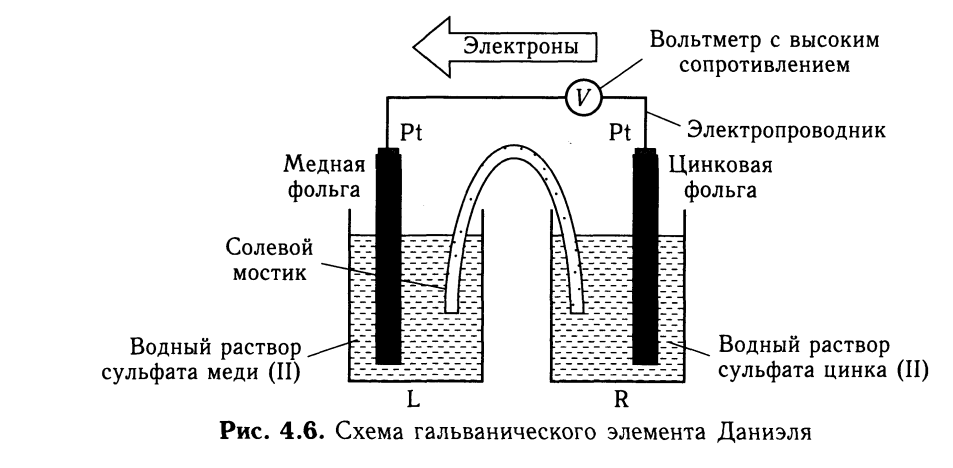
\includegraphics[scale = 0.45]{201}
	\end{figure}
 	Он содержит две сопряженные окислительно-восстановительные пары 
 	\begin{align*}
 	\begin{array}{ll}
 	\mathrm{Zn}^{2+}+2 \mathrm{e} \rightarrow \mathrm{Zn}, & E_{\mathrm{Zn}^{2+} / \mathrm{Zn}}^{\circ}=-0,760 \mathrm{B} \\
 	\mathrm{Cu}^{2+}+2 \mathrm{e} \rightarrow \mathrm{Cu}, & E_{\mathrm{Cu}^{2+} / \mathrm{Cu}}^{\circ}=+0,337 \mathrm{B}
 	\end{array}	
 	\end{align*}
 	Здесь у меди стандартный потенциал выше, значит цинк будет восстановителем, а медь окислителем. Таким образом, цинковый электрод является анодом, медный - катодом. В процессе работы элемента цинк переходит с пластинки в раствор в виде $\mathrm{Zn}^{2+}$, а медь, напротив, осаждается из раствора на пластинку.
 	
 	Для гальванического элемента принята следующая форма записи:
 	$$
 	\mathrm{Zn}\left|\mathrm{ZnSO}_{4} \| \mathrm{CuSO}_{4}\right| \mathrm{Cu}
 	$$
 	где сплошная вертикальная линия | обозначает границу раздела между разными фазами, а двойная сплошная вертикальная линия || - солевой мостик (концентрированный раствор средней соли $-\mathrm{KCl}, \mathrm{KNO}_{3}, \mathrm{NH}_{4} \mathrm{NO}_{3}$ ). Солевой мостик необходим для уменьшения диффузионного потенциала - дополнительной разности потенциалов, которая возникает из-за разной скорости переноса катионов и анионов через границу раздела фаз. Гальванический элемент принято записывать так, чтобы анод находился слева.
 	
 	ЭДС такой системы очевидно равен $E = E_r - E_l$, а если в расчете на 1M действующих реагентов, то просто $E^\circ = E_r^\circ - E_l^\circ$
	
	Гальванические элементы это что-то одноразовое, развернуть реакцию нельзя. Например обычная батарейка. Напротив аккумуляторы можно заряжать. Например свинцовый 
	\begin{align*}
	\mathrm{Pb}\left|\mathrm{H}_{2} \mathrm{SO}_{4}\right| \mathrm{PbO}_{2} \mid \mathrm{Pb}
	\end{align*}
	
	Топливные элементы это те, которые работают долго за счет того, что к ним подводят топливо и уводят отработанные продукты. Типа представлены в табличке.
	\begin{figure}[H]
		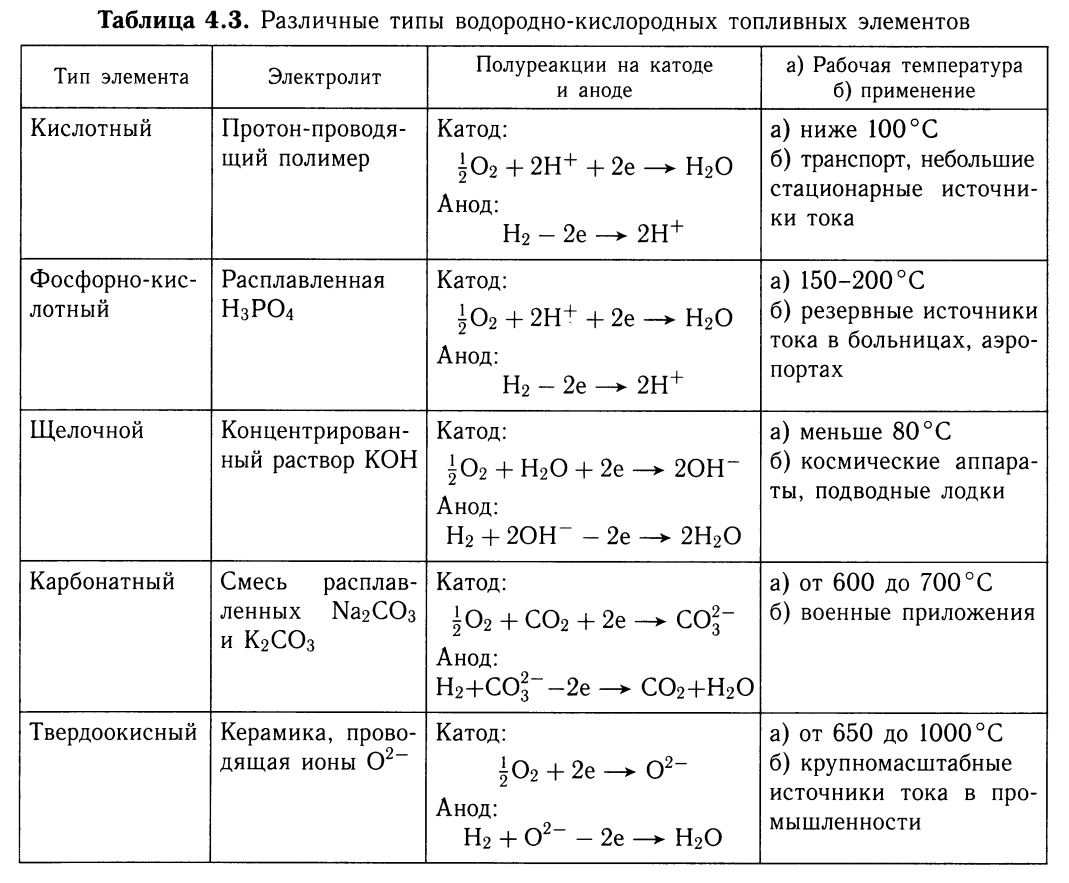
\includegraphics[width=0.7\linewidth]{202}
	\end{figure}
	\subsection{Электролиз}
	\textbf{Электролиз -- окислительно восстановительный процесс, вызванный действием постоянного тока}
	В каком-то смысле это обратный к химическому получению тока процесс. В первом случае мы выкачивали энергию из реакции в цепь, а здесь наоборот закачиваем ее. Поэтому таким образом можно провести даже те реакции, которые вроде бы запрещает термодинамика.
	
	Рассмотрим, например, электролиз расплава $\ce{NaCl}$
	На катоде натрий будет восстанавливаться до металла $\ce{Na^+ + e -> Na}$ а на аноде хлор перейдет в свободное состояние $\ce{2Cl^-  - 2e -> Cl_2}$	
	Таким образом хлорид натрия разлагается на простые вещества.
	
	Если проводить опыт не в расплаве, а в водном растворе, то все немного сложнее. Потому что вода сама может в процессе электролиза разложиться на чистые кислород и водород. Надо понять что будет реагировать первым.
	\begin{align*}
	&\ce{2H_2O + 2e -> H_2 + 2HO^-} &E^0 = - 0.828 V\\
	&\ce{Na^+ + e -> Na}  &E^0  = -2.714V
	\end{align*}
	Как видно вода слабый окислитель, но натрий еще слабее. Поэтому на катоде восстанавливаться будет кислород. На аноде напротив хлор сильнее воды, там будет он будет окисляться. Итого мы получим хлор, водород и щелочь.
	\begin{figure}[H]
		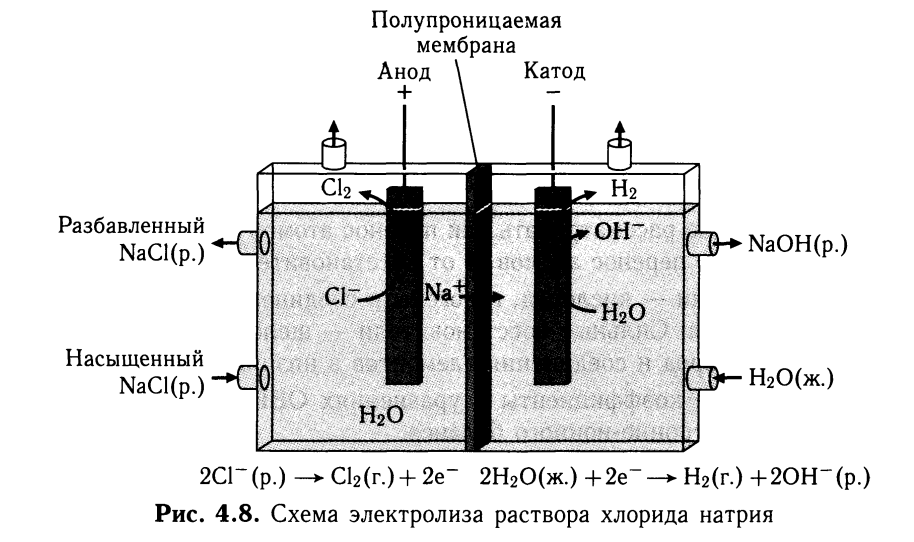
\includegraphics[scale = 0.4]{203}
	\end{figure}